\documentclass[11pt,letterpaper]{article}
\usepackage[T1]{fontenc}
\usepackage{lmodern,microtype}
\usepackage[margin=1in]{geometry}
\usepackage{amsmath,amssymb,amsthm,mathtools}
\usepackage{booktabs,longtable,array,enumitem}
\usepackage[dvipsnames]{xcolor}
\usepackage{tikz}
\usetikzlibrary{arrows.meta}
\usepackage{fancyhdr}
\usepackage[colorlinks=true,linkcolor=MidnightBlue,citecolor=MidnightBlue,urlcolor=MidnightBlue,breaklinks=true]{hyperref}
\usepackage{xurl}
\hypersetup{pdftitle={Beyond Dirichlet GRH: optimal frames and an unramified nonabelian transfer},pdfauthor={Research prepared for Vladimir Reshetnikov}}
\setlength{\emergencystretch}{2.5em}
\setlength{\parskip}{4pt}
\setlength{\parindent}{0pt}
\setlist{itemsep=3pt,topsep=5pt,leftmargin=*}
\pagestyle{fancy}
\fancyhf{}
\fancyhead[L]{\small Beyond Dirichlet GRH}
\fancyhead[R]{\small Research analysis, 25 November 2026}
\fancyfoot[C]{\thepage}
\setlength{\headheight}{14pt}
\newcommand{\Q}{\mathbb Q}
\newcommand{\Z}{\mathbb Z}
\newcommand{\R}{\mathbb R}
\newcommand{\C}{\mathbb C}
\newcommand{\N}{\mathbb N}
\newcommand{\OO}{\mathcal O}
\newcommand{\DD}{\mathfrak D}
\newcommand{\Tr}{\operatorname{Tr}}
\newcommand{\Gal}{\operatorname{Gal}}
\newcommand{\rd}{\operatorname{rd}}
\newcommand{\ord}{\operatorname{ord}}
\newcommand{\Sha}{\mathrm{Sha}}
\newcommand{\pos}[1]{\left(#1\right)_+}
\newcommand{\src}[2]{\href{https://github.com/lsernau/grh-lean/blob/72fead102f663d5c7a407964a13dc0cf9d977207/grh/src/#1.lean}{\texttt{\detokenize{#2}}}}
\newcommand{\prior}[2]{\href{https://github.com/VladimirReshetnikov/ProveIt/blob/28ad287a8d13c0f864ebb51c7c053ad06aa6e585/docs/incoming/#1}{#2}}
\newtheorem{theorem}{Theorem}[section]
\newtheorem{proposition}[theorem]{Proposition}
\newtheorem{lemma}[theorem]{Lemma}
\newtheorem{corollary}[theorem]{Corollary}
\theoremstyle{definition}
\newtheorem{definition}[theorem]{Definition}
\newtheorem{remark}[theorem]{Remark}
\newcolumntype{L}[1]{>{\raggedright\arraybackslash}p{#1}}
\begin{document}
\begin{titlepage}
\vspace*{0.55in}
{\color{MidnightBlue}\large RESEARCH REPORT}\par
\vspace{0.25in}
{\Huge\bfseries Beyond Dirichlet GRH}\par
\vspace{0.16in}
{\LARGE Optimal frames and an unramified\par nonabelian transfer}\par
\vspace{0.35in}
{\large Analysis of \texttt{lsernau/grh-lean}, building on the\par ProveIt incoming research archive}\par
\vspace{0.35in}
Prepared for Vladimir Reshetnikov\par
25 November 2026\par
\vspace{0.45in}
\hrule
\vspace{0.18in}
\textbf{Main result.} The selected real $S_3$ field admits an optimal integral frame of bound $229$ using eight vectors. Its cubic extension of the source's cyclotomic CM field is unramified, so the different and fractional Weil lattice extend without a new ramification cost. A projective Hermitian argument supplies frames of every sufficiently large integer bound in the corrected lattice.

\textbf{Research conclusion.} These results remove qualitative arithmetic obstacles to a nonabelian extension of the method. They do not yet give the scale-uniform frame and odd-cocycle estimates needed to prove a new nonabelian Riemann hypothesis. The remaining estimates are stated precisely.

\textbf{Validation.} Full mathematical proofs and exact integer/rational certificates are included. The upstream Lean source was inspected and statically scanned; its complete Lean build and kernel checks were not rerun here.
\vfill
\small Source: \texttt{72fead102f663d5c7a407964a13dc0cf9d977207}\par
ProveIt: \texttt{28ad287a8d13c0f864ebb51c7c053ad06aa6e585}
\end{titlepage}
\begingroup
\small
\setlength{\parskip}{0pt}
\tableofcontents
\endgroup
\newpage
\section{Answer, scope, and relation to the earlier reports}

The source contains methods worth transferring beyond familiar consequences of RH and Dirichlet GRH. The most promising transfer identified here is to a specific nonabelian number field, rather than to another equivalent analytic criterion. The present work proves new arithmetic inputs relative to the inspected ProveIt reports, corrects an unnecessarily pessimistic assessment of the different in their chosen example, and isolates the quantitative statements still needed. It does not claim to resolve a further named open conjecture.

\subsection{What has been accomplished in this report}

\begin{enumerate}
\item \textbf{An exact optimal frame.} For the real $S_3$ splitting field of $X^3-4X+1$, the earlier frame bound $48\cdot229^2=2{,}517{,}168$ is replaced by the optimal positive integer bound $229$. There are seven displayed vectors, one used twice. The improvement factor is $10{,}992$. Optimality concerns the bound, not the number of vectors.
\item \textbf{A structural obstruction.} Every ordinary integral tight frame in this field has bound divisible by $229$. Thus a new basis or more integral vectors cannot produce coprime bounds in the unchanged ring of integers.
\item \textbf{A favorable unramified extension.} The splitting field is an unramified cyclic cubic extension of $\Q(\sqrt{229})$. Once $229$ is included in the cyclotomic modulus, adjoining the nonabelian field preserves the source's different and root discriminant. The old fractional Weil lattice extends and remains Hermitian self-dual. An internal upstream theorem already supplies compatible Weil data.
\item \textbf{Qualitative frames at all large bounds.} For a self-dual projective Hermitian lattice over an imaginary quadratic ring containing an element of trace one, every sufficiently large integer is a frame bound. The frame can contain any prescribed finite set, with any prescribed lower multiplicity. This removes the need to assume that the lattice is free.
\item \textbf{A weaker sufficient cocycle target.} In the source scaling, the odd-cocycle contribution is negligible if $\log X\le b$; the source's stronger polynomial bound on $\log X$ is not essential for this one error term. This is a conditional budget calculation, not a new bound on the cocycles themselves.
\end{enumerate}

These assertions are proved below. The abstract ingredients have classical antecedents in trace duality, Hermitian forms, and sums of squares. No worldwide priority claim is made. The exact certificates and their application to the selected transfer were not found in the inspected earlier reports. The distinction between a new contribution to this research archive and a new theorem in the literature is maintained throughout.\cite{Milne,BCIL,priorSynthesis}

\subsection{What the repository actually exports}

The source's five public endpoints are Mathlib's \texttt{RiemannHypothesis} and four statements about zeros of the Riemann zeta function and Dirichlet $L$-functions. The character statements cover all positive moduli and all Dirichlet characters, including imprimitive ones. They do not quantify over arbitrary number fields, Hecke characters, Artin representations, or automorphic representations. The statements file imports only Mathlib.\cite{source}

The inspected source is pinned to commit
\begin{center}\texttt{72fead102f663d5c7a407964a13dc0cf9d977207}.\end{center}
It specifies Lean v4.35.0 and Mathlib commit
\texttt{56a005855ea17e0b0958f73ec801ae140b0a1679}.
The repository reports successful machine checks and dependence only on
\texttt{propext}, \texttt{Classical.choice}, and \texttt{Quot.sound}.
Public verification reports give additional supporting evidence. This investigation takes those results as the starting point while distinguishing source inspection from a fresh kernel verification.\cite{source,Sutherland,Sonoda}

A static scan of both source trees found no code occurrences of \texttt{sorry}, \texttt{axiom}, \texttt{admit}, \texttt{unsafe}, \texttt{native\_decide}, \texttt{implemented\_by}, or \texttt{run\_tac}. The readable tree has 803 source files and the compact tree 794; all are reachable from their respective \texttt{Main} module in the local import scan. The comparator's \texttt{Challenge.lean} placeholders are outside those source import closures. A static scan is supplementary evidence and cannot establish successful elaboration, semantics, or kernel acceptance.

\subsection{What was already done in ProveIt}

The inspected ProveIt commit is
\begin{center}\texttt{28ad287a8d13c0f864ebb51c7c053ad06aa6e585}.\end{center}
Its incoming directory contains 32 GRH research archives. The latest synthesis, the five reports outside that synthesis's inventory, and principal sections of three additional predecessors were read directly. The other 23 packages were assessed through the synthesis's claim matrix, not independently re-audited. The package contains the full inventory and inspection record.\cite{priorSynthesis,priorStructural,priorSampling,priorZeroData,priorExact,priorSparse}

\begin{longtable}{@{}L{.25\textwidth}L{.41\textwidth}L{.27\textwidth}@{}}
\toprule
Earlier work & Established or reported contribution & Status in this report\\
\midrule\endhead
Transfer synthesis & Explicit discriminant-229 frame; nonabelian local partner; joint Mellin filters; sharp positive-ramp moment conversion & The frame/global-lattice portion is extended here.\\[5pt]
Exponent-six archive & Completion of the residual interval for 432 imaginary quadratic fields, and 1,236 orders & Earlier result; no rediscovery or fresh full replay claimed here.\\[5pt]
Structural transfers & Exact congruence-module length formula; symmetric mirror image; obstruction to a direct BSD substitution & Reused as a warning against conflating the source modules with standard Selmer ranks.\\[5pt]
Torsion and sampling & Torsion specialization bounds, sparse zero-simplicity and multiplicity criteria & Analytic or specialization interfaces already available; no new prime-side estimate supplied.\\[5pt]
Sparse CM/symmetric powers & Sparse singular-modulus results and optimized nonnegative test polynomials & No new classification claimed in the present work.\\
\bottomrule
\end{longtable}

The main reason to concentrate on a global arithmetic input is that the archive already has numerous detectors, averaged criteria, and finite-group constructions. Another correct zero-detection criterion would leave essentially the same central problem unresolved.

\section{The source mechanism and the transfer interface}

The proof's arithmetic heart compares the same index-corrected covolume from two sides. In schematic notation, with target dimension $d_T$, a family of $n$ independent images, covolume bound $V$, and index cost $\delta$,
\[
 H-\text{error}\ \le\ \frac{V+2\delta}{d_T}
 \ \le\ H-\frac{n}{d_T}m\,\mathrm{rem}+\text{error}.
\]
The main height $H$ cancels. The source obtains $n\ge d_T/2$ and proves
\begin{equation}\label{eq:star}
 m\,\mathrm{rem}\le f a(\log b)^5.
\end{equation}
Here $m$ is the number of lifts, $f$ the number of CM embeddings, and $a=xb$ the main derivative order. The precise comparison is
\src{New/Reduction/MainInequality}{star_inequality}. It depends on short integral source forms, enough independent target images, and a lower bound on the length of integral target forms.\cite{mainInequality}

The resulting weighted prime remainder has the form
\begin{equation}\label{eq:sourceR}
 R_{q,d}(x)=\sum_{\substack{n\le x\\n\equiv1\pmod q}}
 \Lambda(n)(1-\chi_K(n))\left(\frac1n-\frac1x\right)
 -\frac{\log x}{\varphi(q)}-c_{q,d},
\end{equation}
where $K=\Q(\sqrt{-d})$ and $c_{q,d}$ makes the remainder tend to zero. The source establishes the eventual upper bound $R_{q,d}(x)\le x^{-1/2+\varepsilon}$. A Landau argument excludes poles of its transformed remainder to the right of $1/2$. The auxiliary quadratic twist is chosen so that its zeros do not cancel the zeros being detected.\cite{oneSided,criterion,Landau}

This separation identifies what must be transported. The final analytic lemma is general and is explicitly classed as known Landau theory by the source. The difficult transfer is to construct integral objects whose valuations encode the new prime statistic, preserve the normalized height comparison, and control rank and denominators in the required range. A character-table identity alone does not perform that construction.

The earlier discriminant-229 example is well chosen because it allows nonabelian Frobenius information inside the local theta formal group. Its embedding group is a fiber product, not a direct product:
\[
 \Gal(F\Q(\zeta_q)/\Q)
 =\{(g,u)\in S_3\times(\Z/q\Z)^\times:
 \operatorname{sgn}(g)=\chi_{229}(u)\},\qquad229\mid q.
\]
This has order $3\varphi(q)$. The earlier report constructs the corresponding splitting selector and inert-prime partner congruence. The results below address the arithmetic lattice in which those local identities must live.\cite{priorSynthesis}

\section{Optimal integral frames and the ramification obstruction}
\label{sec:frames}

For a totally real number field $F$ of degree $n$, an ordinary integral tight frame of bound $M\in\Z_{>0}$ is a finite family $v_i\in\OO_F$ with positive integer multiplicities $m_i$ such that
\begin{equation}\label{eq:frame}
 \sum_i m_i\sigma(v_i)\tau(v_i)=M\delta_{\sigma,\tau}
 \qquad(\sigma,\tau:F\hookrightarrow\R).
\end{equation}
Thus the vectors give a resolution of a scalar identity in the embedding space. Repeated vectors can replace multiplicities. This is the linear-algebra part of the source's frame input; its global integrality condition instead uses a fractional Weil lattice.

\subsection{Why a ramified prime must divide the bound}

\begin{theorem}[Trace-dual obstruction]\label{thm:dual-obstruction}
If \eqref{eq:frame} holds, then
\begin{equation}\label{eq:codiff-obstruction}
 M\DD_{F/\Q}^{-1}\subseteq\OO_F.
\end{equation}
In particular, every rational prime ramified in $F$ divides $M$.
\end{theorem}

\begin{proof}
Let $a$ lie in the codifferent, so $\Tr_{F/\Q}(a v_i)\in\Z$ for all $i$. Applying the frame operator to the embedding vector of $a$ gives
\[
 M a=\sum_i m_i\Tr_{F/\Q}(a v_i)v_i\in\OO_F.
\]
This proves \eqref{eq:codiff-obstruction}. At a prime $\mathfrak p$ over a ramified rational prime $p$, write $e_{\mathfrak p}$ for the ramification index and $d_{\mathfrak p}>0$ for the different exponent. The ideal containment requires
\[
 e_{\mathfrak p}v_p(M)\ge d_{\mathfrak p},
\]
so $v_p(M)\ge1$.
\end{proof}

The obstruction concerns every ordinary integral frame, not only a particular construction. It also explains why the source allows denominators in one half of the relative codifferent. Those denominators change the dual lattice; they are essential arithmetic data.

\subsection{The exact eventual congruence obstruction for an integral lattice}

The elementary obstruction has a useful converse away from a finite initial range.

\begin{theorem}[Eventual frame bounds for an integral lattice]\label{thm:real-eventual}
Let $L$ be a positive definite integral $\Z$-lattice of positive rank with Gram matrix $G$ in an integral basis. Put
\[
 d=\min\{a\in\Z_{>0}:aG^{-1}\text{ has integer entries}\}.
\]
Every positive integer tight-frame bound for vectors in $L$ is divisible by $d$, and every sufficiently large positive multiple of $d$ is such a bound.
\end{theorem}

\begin{proof}
Let $B$ be the real basis matrix, so $G=B^{\mathsf T}B$. If the frame vectors have integer coordinate columns $u_i$, its identity becomes
\[
 \sum_i m_i u_i u_i^{\mathsf T}=M G^{-1}.
\]
The left side is integral. This proves $d\mid M$; equivalently, $d$ is the exponent of the discriminant group $L^\#/L$.

For sufficiency set $C=dG^{-1}$, a positive definite integral symmetric matrix. The rank-one matrices generated by $e_i$ and $e_i+e_j$ span all integral symmetric matrices over $\Z$: their differences give the off-diagonal matrix units, while $e_ie_i^{\mathsf T}$ gives the diagonal units. Let $S$ be this finite set of vectors. For a sufficiently small positive rational $\epsilon$, the matrix
\[
 C-\epsilon\sum_{v\in S}vv^{\mathsf T}
\]
is positive definite and rational. Rational $LDL^{\mathsf T}$ decomposition expresses it as a sum of positive rational multiples of rational rank-one matrices. Scaling their vectors to integer vectors and clearing coefficients yields
\[
 qC=\sum_{v\in T}c_vvv^{\mathsf T},\qquad c_v\in\Z_{>0},\quad S\subseteq T.
\]
Write $C=\sum_{v\in T}z_vvv^{\mathsf T}$ with $z_v\in\Z$, using $S$, and extending by zero on other vectors. For $n=kq+r$, $0\le r<q$,
\[
 nC=\sum_{v\in T}(kc_v+rz_v)vv^{\mathsf T}.
\]
For all sufficiently large $k$, every coefficient is nonnegative. The resulting frame has bound $nd$. The same argument makes every coefficient exceed any prescribed fixed lower bound.
\end{proof}

This proof supplies an effective threshold once a rational reserve decomposition has been chosen. It supplies no useful uniform bound as the rank and arithmetic data vary. Sums of integral squares and Hermitian norms form an established subject; the present formulation is used as a transfer tool.\cite{BCIL}

\subsection{The cubic field and its optimal six-vector certificate}

Let $f(X)=X^3-4X+1$ and let $\alpha$ be a root. The rational root test proves irreducibility. There is a root in each of $(-3,-2)$, $(0,1)$, and $(1,2)$, so the cubic field $F_0=\Q(\alpha)$ is totally real. Its polynomial discriminant is
\[
 -4(-4)^3-27=229,
\]
a prime. Thus $(1,\alpha,\alpha^2)$ is an integral basis, and the trace Gram matrix is
\[
 T=\begin{pmatrix}3&0&8\\0&8&-3\\8&-3&32\end{pmatrix},
 \qquad
 229T^{-1}=\begin{pmatrix}247&-24&-64\\-24&32&9\\-64&9&24\end{pmatrix}.
\]
Newton sums give $\Tr(1),\Tr(\alpha),\ldots,\Tr(\alpha^4)=(3,0,8,-3,32)$.

The following coordinate vectors have outer products summing to $229T^{-1}$:
\begin{center}
\begin{tabular}{@{}rrrcr@{}}
\toprule
$1$&$\alpha$&$\alpha^2$&&Multiplicity\\\midrule
0&2&1&&1\\
1&-1&1&&2\\
2&-1&1&&1\\
4&-5&-2&&1\\
15&0&-4&&1\\\bottomrule
\end{tabular}
\end{center}
Therefore they give a six-vector frame of bound $229$. Theorem~\ref{thm:dual-obstruction} shows that no smaller positive integer bound is possible. No assertion about a minimum number of vectors is needed.

\subsection{The $S_3$ field and an optimal eight-vector certificate}

Let $F$ be the splitting field and let $\alpha,\beta$ be distinct roots of $f$. Its Galois group is $S_3$, because the irreducible cubic has nonsquare discriminant. Its six embeddings correspond to ordered pairs of distinct roots. Define
\[
 b=(1,\alpha,\alpha^2,\beta,\alpha\beta,\alpha^2\beta).
\]
This is an integral basis. Here is a direct discriminant justification, also useful below. Only $229$ can ramify in the splitting field. At $229$ the extension is tame, and
\[
 f(X)\equiv(X-29)^2(X+58)\pmod{229}.
\]
Inertia has order two and acts as a transposition: it is nontrivial, cyclic, and fixes the simple-root branch. A tame degree-six Galois extension with inertia index two has discriminant exponent $6(1-1/2)=3$. Consequently $\operatorname{disc}(F)=229^3$. The Gram matrix of $b$, computed below, also has determinant $229^3$, proving that the integral lattice it generates has index one in $\OO_F$.

Write $s_j$ for the $j$th power sum of the three roots. Then
\[
 s_0=3,\quad s_1=0,\quad s_2=8,\qquad
 s_j=4s_{j-2}-s_{j-3}\quad(j\ge3).
\]
For monomials $\alpha^i\beta^j$ and $\alpha^k\beta^l$, their trace product equals
\[
 s_{i+k}s_{j+l}-s_{i+j+k+l}.
\]
It follows that the Gram matrix and its scaled inverse are
\begin{align*}
G&=\begin{pmatrix}
6&0&16&0&-8&3\\
0&16&-6&-8&3&-32\\
16&-6&64&3&-32&20\\
0&-8&3&16&3&32\\
-8&3&-32&3&32&-4\\
3&-32&20&32&-4&125
\end{pmatrix},\\[3pt]
C:=229G^{-1}&=\begin{pmatrix}
125&-16&-32&4&0&-3\\
-16&32&3&0&-3&8\\
-32&3&16&-3&8&0\\
4&0&-3&32&-6&-8\\
0&-3&8&-6&16&0\\
-3&8&0&-8&0&6
\end{pmatrix}.
\end{align*}

\begin{theorem}[Optimal discriminant-229 frame]\label{thm:optimal229}
Let $v_i$ have the following coordinates in $b$, with multiplicities $m_i$:
\begin{center}
\begin{tabular}{@{}rrrrrrcr@{}}
\toprule
$1$&$\alpha$&$\alpha^2$&$\beta$&$\alpha\beta$&$\alpha^2\beta$&&$m_i$\\\midrule
0&2&-2&-2&-1&1&&1\\
1&-2&-2&4&-2&-1&&1\\
2&2&0&1&2&1&&1\\
4&1&-1&1&-1&0&&2\\
4&1&-1&2&0&-1&&1\\
6&-4&-1&-1&2&-1&&1\\
6&-1&-2&-2&-1&1&&1\\\bottomrule
\end{tabular}
\end{center}
They satisfy \eqref{eq:frame} with $M=229$, and $229$ is the smallest possible positive integer bound for any ordinary integral frame in $F$.
\end{theorem}

\begin{proof}
Let $u_i$ denote the displayed columns. Direct integer multiplication gives
\[
 \sum_i m_i u_i u_i^{\mathsf T}=C,
 \qquad GC=229I_6.
\]
If $B=(\sigma(b_j))_{\sigma,j}$, then $B^{\mathsf T}B=G$, whence
\[
 \sum_i m_i\sigma(v_i)\tau(v_i)
 =(BCB^{\mathsf T})_{\sigma,\tau}=229\delta_{\sigma,\tau}.
\]
The vectors are integral. Every positive integer frame bound is divisible by the ramified prime $229$, by Theorem~\ref{thm:dual-obstruction}. This proves optimality.
\end{proof}

The squared trace norms are, in order,
\[
 (221,229,229,74,157,211,179),
\]
and their multiplicity-weighted sum is $6\cdot229$. In particular all real conjugates of every displayed vector have absolute value at most $\sqrt{229}$. The exact checker recomputes the Newton sums, matrices, determinants, outer products, and identities. A numerical search was used only to discover candidate integer columns; no numerical optimizer is part of the verification.

\begin{corollary}[Cyclotomic tensor frame]
For $229\mid q$, the elements $v_i\zeta_q^j$, $0\le j<q$, with the same multiplicities, give a frame of bound $229q$ on the compatible embeddings of $F\Q(\zeta_q)$. The same embedding identity holds on the induced CM type after adjoining the source's imaginary quadratic field $K$.
\end{corollary}

\begin{proof}
Multiply \eqref{eq:frame} by the geometric-sum identity
\[
 \sum_{j=0}^{q-1}\eta(\zeta_q^j)\overline{\eta'(\zeta_q^j)}
 =q\delta_{\eta,\eta'}.
\]
Embeddings of the compositum correspond to compatible pairs of embeddings. Restricting the product identity to those pairs proves the assertion; linear disjointness is not assumed.
\end{proof}

The tensor frame improves an explicit arithmetic constant and preserves integrality at the inert primes used in the earlier local argument. Its bound still carries $229$. The correction needed for coprime bounds is a change to the appropriate fractional lattice, addressed next.

\section{An unramified nonabelian extension of the source field}
\label{sec:unramified}

\subsection{The degree-three extension costs no new different}

Let $k=\Q(\sqrt{229})$. It is the quadratic subfield of the $S_3$ splitting field $F$. The elementary ramification calculation above gives a particularly favorable arithmetic situation.

\begin{theorem}[Unramified cubic base change]\label{thm:unramified}
The extension $F/k$ is cyclic of degree three and unramified at every finite prime. Let $q$ be divisible by $229$ and let $K$ be the imaginary quadratic field from the source. Set
\[
 E_0=K\Q(\zeta_q),\qquad E=F E_0.
\]
Then $[E:E_0]=3$, this extension is unramified at every finite prime, and
\begin{equation}\label{eq:different-inherited}
 \DD_{E/K}=\DD_{E_0/K}\OO_E,\qquad
 \DD_{E/\Q}=\DD_{E_0/\Q}\OO_E,\qquad
 \rd(E)=\rd(E_0).
\end{equation}
\end{theorem}

\begin{proof}
The subgroup fixing $k$ is $A_3$, so $F/k$ is cyclic cubic. Away from $229$ the splitting field is unramified. At $229$ its inertia group is a transposition subgroup of $S_3$, whose intersection with $A_3$ is trivial. Relative inertia for $F/k$ is exactly that intersection. Thus the relative different is the unit ideal.

The quadratic field $k$ has conductor $229$, so it lies in $\Q(\zeta_q)$. The field $E_0/\Q$ is abelian. Therefore $F\cap E_0$ is an abelian Galois subextension of $F/\Q$, and is contained in $k$; since it contains $k$, equality holds. Hence $[E:E_0]=3$.

An unramified extension of local fields remains an unramified finite etale algebra after base change; each field factor is unramified. Apply this at all finite places to $F/k$. This gives $\DD_{E/E_0}=\OO_E$. Transitivity of the different gives the first two identities in \eqref{eq:different-inherited}. The relative discriminant formula gives
\[
 |\operatorname{disc}(E)|=|\operatorname{disc}(E_0)|^3,
\]
and $[E:\Q]=3[E_0:\Q]$, proving the root-discriminant identity.
\end{proof}

\begin{figure}[htbp]
\centering
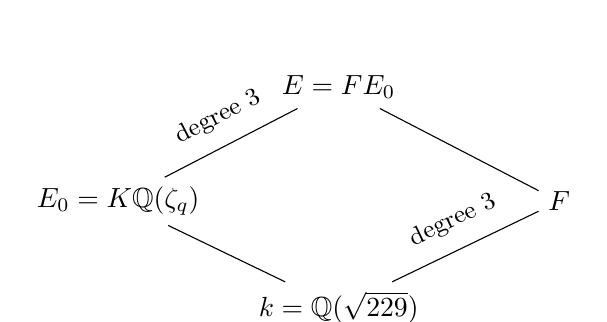
\begin{tikzpicture}[>=Stealth,every node/.style={align=center}]
\node (E) at (0,2.8) {$E=F E_0$};
\node (E0) at (-2.8,1.35) {$E_0=K\Q(\zeta_q)$};
\node (F) at (2.8,1.35) {$F$};
\node (k) at (0,0) {$k=\Q(\sqrt{229})$};
\draw (E0) -- node[above=3pt,midway,font=\small,sloped] {degree $3$} (E);
\draw (F) -- (E);
\draw (k) -- (E0);
\draw (k) -- node[above=3pt,midway,font=\small,sloped] {degree $3$} (F);
\end{tikzpicture}
\caption{The favorable nonabelian benchmark, with $F\cap E_0=k$. Both displayed degree-three extensions are unramified at every finite prime.}
\end{figure}

This corrects the general different-related uncertainty in the earlier synthesis for its specific example. A principal generator of the old different remains a generator after extension. This statement does not say that an arbitrary fractional ideal is principal, or that adjoining an arbitrary nonabelian field has the same property.

\subsection{The fractional lattice and trace self-duality}

From this point on, let $q$ be an admissible source tower modulus, with $229$ included in its fixed base modulus. Let $A_0$ be the source's fractional Weil lattice. In ideal notation its local construction gives
\begin{equation}\label{eq:half-different}
 A_0\overline{A_0}=\DD_{E_0/K}^{-1}.
\end{equation}
It permits inverse-different denominators on one side of each selected conjugate pair of primes, and remains integral on the other side. This is described explicitly by
\src{New/Derivatives/Vacuum/ShortVectors}{finiteImage_mem_iff} and the finite-idele valuation identity in
\src{New/Derivatives/Field/WeilData}{v_alpha_mul_star_mul_relDifferentGen}.\cite{shortVectors,weilField}

For the positive definite Hermitian pairing
\[
 h(x,y)=\Tr_{E/K}(\overline{x}y),
\]
the dual of a fractional ideal $A$ is
\begin{equation}\label{eq:hermitian-dual}
 A^\#=\DD_{E/K}^{-1}\overline A^{-1}.
\end{equation}
Indeed, $h(z,A)\subseteq\OO_K$ is equivalent to
$\overline z A\subseteq\DD_{E/K}^{-1}$; conjugate this condition and use conjugation stability of the different. Trace duality and different transitivity are standard number-field facts.\cite{Milne}

\begin{corollary}[The corrected lattice]
The ideal $A=A_0\OO_E$ satisfies
\[
 A\overline A=\DD_{E/K}^{-1},\qquad A^\#=A.
\]
It is a full projective $\OO_K$-lattice in $E$, with its positive definite Hermitian trace pairing.
\end{corollary}

\begin{proof}
Extend \eqref{eq:half-different} to $\OO_E$ and apply Theorem~\ref{thm:unramified}. Equation~\eqref{eq:hermitian-dual} gives self-duality. A fractional ideal is finite and torsion-free over the Dedekind domain $\OO_K$, hence projective. Under the induced CM type, the trace of $\overline x x$ is a sum of squared complex absolute values, proving positivity.
\end{proof}

For clarity, a more general ideal construction is also available. If every rational prime below $\DD_{E/K}$ splits in $K$, choose one of its two $K$-primes. Put valuation $-v_{\mathfrak P}(\DD_{E/K})$ in $A$ above the chosen prime and valuation zero above its conjugate. Then $A\overline A=\DD_{E/K}^{-1}$ prime by prime. If $E/K$ is Galois, this choice is stable under that Galois group. No principal different is required. The special unramified benchmark is stronger because it reuses the old lattice directly.

\subsection{An existing source theorem supplies the Weil data}

An important internal theorem was absent from the earlier transfer discussion:
\begin{center}
\src{Lib/ClassField/Grunwald}{New.nonempty_weilData_of_not_dvd_differentIdeal}.
\end{center}
It says that a CM extension with compatible CM types inherits Weil data when no finite prime fixed by conjugation divides the relative different. Its proof retains the purely imaginary parameter $j$, pulls the splitting character along the idele norm, and constructs a compatible finite idele.\cite{grunwald}

Theorem~\ref{thm:unramified} verifies the hypothesis in the strongest possible way. Here one can retain the old finite idele by extension, because the different is unchanged. The remaining structural conditions also transport: the root of unity of order $5040$ already lies in the base, the parameter $j$ has the same positive imaginary values on the induced CM type, and its trace-one algebraic integer remains integral. The splitting character is the original one composed with the idele norm $E\to E_0$.

This is an application of an existing theorem in the proof library. It must not be counted as a newly proved general theorem or as a newly compiled Lean instantiation.

\subsection{Period normalization and the old unit witnesses}

The source frame construction needs more than the matrix identity. For each $p$-adic embedding, at least one frame member $y$ must make all of its normalized CM-coordinate coefficients units. In the source, the two possible witnesses are
\begin{equation}\label{eq:unit-witnesses}
 1,\qquad
 \zeta_q\,\mathrm{dualVector}(\varphi(q)-1).
\end{equation}
Their property is the norm assertion
\[
 \left|\iota_p\bigl(c\,\overline{\tau(y)}\bigr)\right|_p=1
 \quad\text{for every CM embedding }\tau,
\]
with the source's period normalization $c$.\cite{shortVectors,tightFrames}

Every new CM embedding restricts to an old one. The finite-idele valuations and root discriminant extend unchanged. Consequently the same norm assertions hold for the two old witnesses in $A$.

There is a normalization subtlety. The source defines its vacuum root by a principal complex root. Under degree-three base change, the quantity whose root is taken is cubed and the root degree triples. Recomputing the principal root need not give the same complex number: the new and old choices can differ by a root of unity. Their absolute values at all archimedean and $p$-adic places agree. Alternatively, choose the inherited old root as the new normalization; it satisfies the new power equation. Thus the unit-witness statement transports as an equality of norms. Literal equality of independently chosen principal-root values is not asserted.

The witnesses alone cannot span the new embedding directions. The next section proves that one can include them in genuine frames at every sufficiently large integer bound, without assuming a free lattice.

\section{Every sufficiently large bound in the corrected lattice}
\label{sec:projective}

The key distinction is now between qualitative existence and the uniform estimates required by the source. We can prove the former in a general projective setting.

\subsection{Statement}

Let $K$ be imaginary quadratic, $\OO=\OO_K$, and assume that some $\eta\in\OO$ satisfies
\begin{equation}\label{eq:traceone}
 \eta+\overline\eta=1.
\end{equation}
For the source, $K=\Q(\sqrt{-d})$ with $d\equiv7\pmod8$, and $\eta=(1+\sqrt{-d})/2$ works. Let $V$ have positive dimension over $K$, and let $h$ be positive definite Hermitian, conjugate-linear in the first variable. For $v\in V$, define the rank-one operator
\[
 \Theta_v(z)=v h(v,z).
\]
For $x,y\in V$, also put $\Theta_{x,y}(z)=x h(y,z)$.

\begin{theorem}[Projective Hermitian eventual frames]\label{thm:projective}
Let $A$ be a full projective $\OO$-lattice in $V$ with $A^\#=A$. Let $S\subset A$ be finite and $R\in\Z_{\ge0}$. There are a fixed finite family $T\subset A$ containing $S$ and an integer $M_0$ such that for every integer $M\ge M_0$ there are integers $m_v\ge R$ satisfying
\begin{equation}\label{eq:projective-frame}
 \sum_{v\in T}m_v\Theta_v=M I_V.
\end{equation}
In orthonormal complex coordinates this is an ordinary tight-frame identity. Neither freeness of $A$ nor a principal fractional ideal is assumed.
\end{theorem}

\subsection{Step 1: an integral signed resolution of the identity}

\begin{lemma}\label{lem:signed}
Under the hypotheses of Theorem~\ref{thm:projective}, the identity is an integer linear combination of finitely many $\Theta_v$ with $v\in A$.
\end{lemma}

\begin{proof}
The dual-basis lemma for a finite projective module supplies $x_i\in A$ and $\OO$-linear functionals $\ell_i:A\to\OO$ such that
\[
 z=\sum_i x_i\ell_i(z).
\]
Each functional extends to $V$ and, by nondegeneracy, has the form $\ell_i(z)=h(y_i,z)$ for some $y_i\in V$. Since $\ell_i(A)\subseteq\OO$, self-duality implies $y_i\in A$. Thus
\[
 \sum_i\Theta_{x_i,y_i}=I,
 \qquad \sum_i\Theta_{y_i,x_i}=I,
\]
where the second equality is the adjoint of the first.

Direct expansion gives the exact polarization identity
\begin{equation}\label{eq:polarization}
 \Theta_{x+\eta y}-\Theta_x-N_{K/\Q}(\eta)\Theta_y
 =\overline\eta\,\Theta_{x,y}+\eta\,\Theta_{y,x}.
\end{equation}
Summing over $i$ and applying \eqref{eq:traceone} gives $I$ on the right. The left is an integer linear combination of rank-one operators of lattice vectors, since $N_{K/\Q}(\eta)\in\Z$. Combine repeated vectors to obtain
\begin{equation}\label{eq:signed-id}
 I=\sum_{v\in S'}z_v\Theta_v,\qquad z_v\in\Z.
\end{equation}
The prescribed set $S$ can be added to $S'$ with zero coefficients.
\end{proof}

The trace-one element removes the factor two that a purely real polarization argument would introduce. Projective dual generators replace a global integral basis; this is why no freeness assumption enters the proof.

\subsection{Step 2: a positive reserve containing prescribed vectors}

\begin{lemma}\label{lem:reserve}
For every finite $S'\subset A$, there are a positive integer $q$, a finite $T\supseteq S'$, and positive integers $c_v$ such that
\begin{equation}\label{eq:reserve}
 q I=\sum_{v\in T}c_v\Theta_v.
\end{equation}
\end{lemma}

\begin{proof}
Choose a sufficiently small positive rational $\epsilon$ so that
\[
 I-\epsilon\sum_{v\in S'}\Theta_v
\]
is positive definite. Choose a $K$-basis of $V$ inside $A$, with complex coordinate matrix $B$. Its Hermitian Gram matrix $H=B^*B$ has entries in $K$. If $u_v\in K^n$ is the coordinate column of $v$, then
\[
 I=BH^{-1}B^*,\qquad \Theta_v=Bu_vu_v^*B^*.
\]
The residual matrix
\[
 H^{-1}-\epsilon\sum_{v\in S'}u_vu_v^*
\]
is positive definite Hermitian over $K$. Hermitian $LDL^*$ decomposition has a triangular factor over $K$ and strictly positive diagonal entries in $K\cap\R=\Q$. This expresses the residual as a sum of positive rational multiples of rank-one matrices with vectors in $K^n$.

Multiply each vector by an integer so that its image in $V$ lies in $A$, and divide its coefficient by the corresponding square. Reinsert the vectors of $S'$ with coefficient $\epsilon$. Clearing all positive rational denominators gives \eqref{eq:reserve}. Zero vectors, if prescribed, may be retained with arbitrary positive coefficients. Combine duplicate vectors if necessary.
\end{proof}

\subsection{Step 3: absorb the signed coefficients}

\begin{proof}[Proof of Theorem~\ref{thm:projective}]
Use \eqref{eq:signed-id} and \eqref{eq:reserve}, extending $z_v=0$ outside the signed support. Define
\begin{equation}\label{eq:explicit-threshold}
 k_0=\max_{v\in T}
 \left\lceil\frac{R+(q-1)\max(0,-z_v)}{c_v}\right\rceil,
 \qquad M_0=qk_0.
\end{equation}
For $M\ge M_0$, write $M=kq+r$ with $0\le r<q$. Set
\[
 m_v=kc_v+rz_v.
\]
Then $k\ge k_0$ and every $m_v\ge R$. Moreover,
\[
 \sum_{v\in T}m_v\Theta_v
 =k\sum_{v\in T}c_v\Theta_v+r\sum_{v\in T}z_v\Theta_v
 =kqI+rI=MI.
\]
This proves the theorem with a fixed family independent of $M$.
\end{proof}

\begin{corollary}[Coprime and prescribed large bounds]
The corrected ideal $A=A_0\OO_E$ from Section~\ref{sec:unramified} has frames of every sufficiently large positive integer bound. In particular it has coprime pairs of bounds, and arbitrarily large bounds prime to any fixed integer. One can prescribe both old unit witnesses \eqref{eq:unit-witnesses} as frame members with any fixed lower multiplicity.
\end{corollary}

\begin{proof}
The ideal is Hermitian self-dual and projective, and $\OO_K$ contains the required trace-one element. Apply Theorem~\ref{thm:projective}. Consecutive sufficiently large integers give coprime bounds; integers congruent to one modulo a fixed integer give the other assertion.
\end{proof}

\subsection{A general finite local-unit witness principle}

The inherited two-element witness set is unusually convenient. A qualitative substitute exists for any fractional ideal.

\begin{lemma}[Finite simultaneous local generators]\label{lem:local-generators}
For a nonzero fractional ideal $A$ of a number field $E$, there is a finite set $S\subset A$ such that, for every rational prime $p$, some $y\in S$ satisfies
\[
 v_{\mathfrak P}(y)=v_{\mathfrak P}(A)
 \quad\text{for all }\mathfrak P\mid p.
\]
\end{lemma}

\begin{proof}
Choose $0\ne y_0\in A$. The integral ideal $(y_0)A^{-1}$ has finite support. Outside the finitely many rational primes below that support, $y_0$ already works. For each exceptional $p$, choose a nonzero class in every one-dimensional residue module $A/\mathfrak P A$, for $\mathfrak P\mid p$. The Chinese remainder theorem gives one element $y_p\in A$ representing those classes simultaneously. Its local valuation is exactly that of $A$ at every such prime. Take $S$ to consist of $y_0$ and these finitely many $y_p$.
\end{proof}

If $A$ is $\Gal(E/K)$-stable, one such element has the analogous simultaneous normalized-unit property under all $K$-embeddings, relative to local trivializations of $A$. A comparison with a particular global period normalization is still required. In our unramified benchmark the inherited source witnesses already satisfy that comparison as norm assertions.

\subsection{What this theorem does and does not settle}

For each fixed tower level, qualitative coprime frames and prescribed sufficiently large bounds are now available in the correct lattice. The earlier raw integral frame obstruction is therefore overcome by the fractional-lattice construction, not contradicted.

The proof deliberately records its threshold \eqref{eq:explicit-threshold}. It may be very large. Rational decomposition and denominator clearing do not by themselves bound $q$, $c_v$, $z_v$, the coordinates of the vectors, or $M_0$ uniformly in a growing tower. The source needs a small auxiliary bound $h\le b$ and exact final bound $M=p_0p_1$ in a prescribed window, with multiplicities at least $6fb$ and controlled conjugate norms. None of these quantitative inequalities follows from qualitative eventual existence. Establishing them is the first remaining substantial theorem.

\section{The remaining estimates and a concrete new zero problem}
\label{sec:remaining}

\subsection{Why the qualitative frame theorem does not finish the transfer}

The source's scale hierarchy is unusually demanding. For every fixed sufficiently small $\varepsilon>0$, it takes
\[
 m\asymp\sqrt x,\quad r\asymp x^5,\quad t=5r,
 \quad \log b\asymp x^\varepsilon,
 \quad f\ge\varphi(q_0)x^{11}.
\]
The tower modulus has polynomial growth in $x$ up to logarithmic factors. The construction must work for arbitrarily small positive $\varepsilon$ to reach the critical line.\cite{guide,oneSided}

Theorem~\ref{thm:projective} allows arbitrary dependence on the field, lattice, and prescribed witnesses. If its threshold grew as $\exp(f^c)$ for a fixed $c>0$, it would generally exceed the permitted scale $b=\exp(x^\varepsilon)$ when $\varepsilon$ is small. Choosing $b$ still larger would also change the error in \eqref{eq:star}; the limits cannot be adjusted independently.

The next useful frame theorem must control the reserve denominator, signed coefficients, vector sizes, and threshold uniformly as $q$ grows. A polynomial bound in $q$ with fixed exponents would be a very favorable outcome. A proof of mere finite generation or eventual existence is insufficient. In particular, neither the factor-three field extension nor the improved constant $229$ proves those uniform bounds automatically.

\subsection{The exact odd-cocycle obstruction}

The source theorem
\src{Lib/Cyclotomic/OddSha}{New.exists_length_shaOdd_le}
requires the entire CM field to lie in a cyclotomic field $\Q(\mu_N)$. It produces one nonzero integer $X$ with
\begin{equation}\label{eq:odd-source}
 X\le 2^{4(N+t+3)^{27}}h_E
\end{equation}
whose valuations bound the lengths of all the relevant finite-level modules, uniformly over the indicated weights and coefficient rings.\cite{oddSha}

The enlarged field contains the nonabelian $S_3$ field $F$, so that cyclotomic containment is impossible. Unramifiedness over $E_0$ does not make $E/\Q$ abelian. Further, the module in question is a specifically defined module of raw cocycles with local conditions; for positive weights it is not a quotient by coboundaries. The source explicitly provides no comparison with the customary $\Sha^1$ model. Known Iwasawa or $K$-theoretic finiteness results cannot simply be inserted without proving the comparison and the required quantitative uniformity.\cite{oddSha,selmerModules}

The unramified cyclic cubic structure suggests a sharper organizing strategy. In ordinary cohomology, away from the coefficient prime $3$, restriction and corestriction identify the invariant part with the base-field contribution. After adjoining cubic roots of unity to coefficients, the two other eigenspaces involve the two nontrivial cubic characters of $E/E_0$. Those pieces are not controlled by the invariant part. The natural next question concerns corresponding finite-order character twists over the cyclotomic base, with a separate analysis at $3$. This is an organizing observation for genuine cohomology; its comparison with the source's raw cocycles and local conditions remains to be proved.

\subsection{A weaker sufficient quantitative target}

The source's final denominator budget is
\begin{equation}\label{eq:budget}
 \mathcal B=\frac{fa(\log b)^3}{mk}.
\end{equation}
The odd-cocycle part contributes $t\log X$ after summing its prime valuations with weights $\log\ell$. The source bounds $\log X$ by $x^{2000}$, but this is stronger than the budget requires.\cite{fitTwists,traceRelations}

\begin{proposition}[Permissible odd-cocycle growth]\label{prop:budget}
Suppose $x>1$, $b\ge e$, $q_0\ge1$, all of $m,k,r,t,f,a$ are positive, and the transferred data satisfy
\[
 t=5r,\quad r\le3x^5,\quad k\le r,\quad m\le2\sqrt x,
 \quad f\ge\varphi(q_0)x^{11},\quad a=xb.
\]
For $X\ge1$,
\begin{equation}\label{eq:budget-ratio}
 \frac{t\log X}{\mathcal B}
 \le \frac{90}{\varphi(q_0)}x^{-3/2}
 \frac{\log X}{b(\log b)^3}.
\end{equation}
In particular, $\log X\le b$ makes this contribution negligible as $x\to\infty$.
\end{proposition}

\begin{proof}
The scale inequalities give $tmk\le5r^2m\le90x^{21/2}$ and $fa\ge\varphi(q_0)x^{12}b$. Substitute these in $tmk\log X/[fa(\log b)^3]$. The exponent difference is $21/2-12=-3/2$, proving \eqref{eq:budget-ratio}. Under $\log X\le b$, the right side tends to zero.
\end{proof}

For every fixed $\varepsilon>0$ with $\log b\asymp x^\varepsilon$, even a uniform bound $\log X\le\exp(x^{o(1)})$ suffices asymptotically for this term. This relaxes the next arithmetic target. It does not bound the new modules, settle the prime $3$, or account for all other denominator terms.

\subsection{The first nonabelian analytic target}

Let $\rho$ denote the standard two-dimensional representation of $S_3$. The regular-representation factorization is
\begin{equation}\label{eq:zeta-F}
 \zeta_F(s)=\zeta(s)L(s,\chi_{229})L(s,\rho)^2.
\end{equation}
The representation $\rho$ is induced from either nontrivial character of $A_3$. Its $L$-function is a Hecke $L$-function over the real quadratic field $k=\Q(\sqrt{229})$, attached to the unramified cubic extension $F/k$. Its holomorphy is already covered by the classical theory of nontrivial finite-order Hecke characters; this is not a new Artin-holomorphy claim. Its critical-line zero statement is outside the endpoints of the inspected repository.\cite{Milne,source}

For a direct positive statistic write
\[
 -\frac{\zeta_F'}{\zeta_F}(s)=\sum_{n\ge1}a_F(n)n^{-s},
 \qquad
 \zeta_F(s)=\frac{\kappa_F}{s-1}+\kappa_F\gamma_F+O(s-1).
\]
The Euler factors give $0\le a_F(n)\le6\Lambda(n)$. At an unramified prime,
\[
 a_F(p^j)=6\log p\;\mathbf1_{\operatorname{Frob}_p^j=1}.
\]
Thus these coefficients encode complete nonabelian splitting, not just a congruence class. Define
\begin{equation}\label{eq:targetR}
 R_F(x)=\sum_{n\le x}a_F(n)\left(\frac1n-\frac1x\right)
 -\log x+1+\gamma_F.
\end{equation}
The coefficient bound gives $R_F(x)=O((\log x)^2)$, so its initial Mellin transform $\mathcal F(s)=\int_1^\infty R_F(x)x^{-s}\,dx$ converges for $\Re s>1$. Termwise integration gives
\begin{equation}\label{eq:target-transform}
 \mathcal F(s)=
 -\frac{\zeta_F'(s)/\zeta_F(s)}{s(s-1)}
 -\frac1{(s-1)^2}+\frac{1+\gamma_F}{s-1}.
\end{equation}
The singularity at $1$ is removable. At a zero $\omega$ of multiplicity $m_\omega$ in $\Re s>0$, the residue is
\[
 \operatorname{Res}_{s=\omega}\mathcal F(s)
 =\frac{m_\omega}{\omega(1-\omega)}.
\]
It is positive at real zeros in $(0,1)$.

\begin{proposition}[A sufficient final arithmetic estimate]\label{prop:target}
If, for every $\varepsilon>0$ and every sufficiently large dyadic $Y$,
\begin{equation}\label{eq:target-mean}
 \int_Y^{2Y}\pos{R_F(x)}\,dx\ll_\varepsilon Y^{1/2+\varepsilon},
\end{equation}
then every nontrivial zero of $\zeta_F$ lies on $\Re s=1/2$. Consequently the same is true for the Hecke factor $L(s,\rho)$ in \eqref{eq:zeta-F}.
\end{proposition}

\begin{proof}
For every real $\sigma>1/2$, choose $\varepsilon<\sigma-1/2$ and sum \eqref{eq:target-mean} over dyadic intervals. It follows that the Mellin integral of the positive part converges in $\Re s>1/2$.

Here is the positive-part Landau argument already used in the earlier reports. Let $H$ be the holomorphic Mellin transform of $R_F^+$. Initially $H-\mathcal F$ is the Mellin transform $G$ of the nonnegative negative part $R_F^-$. Its convergence abscissa is at most $1$, by the preceding growth bound. If that abscissa $c$ were greater than $1/2$, the meromorphic continuation would have at most a simple real pole there, with residue equal to the negative of the residue of $\mathcal F$, hence nonpositive. At $c=1$ the latter is regular; in $(1/2,1)$ its real residues are nonnegative. But $G(\sigma)\ge0$ for real $\sigma>c$, so a nonzero simple-pole residue there must be positive. The singularity is therefore removable, contradicting Landau's theorem for a nonnegative Mellin transform at its finite convergence abscissa. Thus $G$ also converges in $\Re s>1/2$, making $\mathcal F=H-G$ holomorphic there.

Every zero of $\zeta_F$ to the right of $1/2$ would give a nonzero pole of \eqref{eq:target-transform}; none exists. The functional equation gives the critical line. Since the other factors in \eqref{eq:zeta-F} have no poles in the open critical strip, any off-line zero of $L(s,\rho)$ would be a zero of $\zeta_F$.
\end{proof}

This is a reused analytic interface, not a new theorem about zeros proved here. The source's local theta construction naturally first produces an auxiliary quadratic-twist difference. Reaching \eqref{eq:target-mean} directly, or proving the required no-cancellation/twist-selection analogue, is another task. The Dirichlet-specific auxiliary twist theorem cannot be transferred by changing notation alone.\cite{priorSynthesis,criterion}

\subsection{Revised research priorities}

\begin{longtable}{@{}L{.26\textwidth}L{.34\textwidth}L{.33\textwidth}@{}}
\toprule
Package & What is now available & Exact remaining work\\
\midrule\endhead
Different and Weil data & Unramified cubic base change; inherited different, root discriminant, lattice and period norms; upstream extension theorem & Formal Lean instantiation and consistent normalizations throughout the enlarged construction.\\[5pt]
Frames and local witnesses & Optimal raw frame $229$; projective frames at every sufficiently large integer bound; old unit witnesses included & Bounds uniform in the growing tower, especially $h\le b$, vector norms, and the final prescribed level.\\[5pt]
Odd cocycles & Exact source module and cost identified; weaker sufficient budget \eqref{eq:budget-ratio} & Uniform integer $X$ for the nonabelian field, with the correct raw local conditions and coefficient-ring quantifiers.\\[5pt]
Prime levels and local losses & Nonabelian splitting selector and local partner from the earlier report & Actual split/principal primes in the required windows, and crystalline-defect and arithmetic spanning estimates.\\[5pt]
Final zero argument & Landau interfaces and explicit nonabelian statistic & A new arithmetic bound such as \eqref{eq:target-mean}, or a matched auxiliary-twist version with cancellation excluded.\\
\bottomrule
\end{longtable}

The most efficient next attempt is a quantitative frame construction for this unramified cubic tower together with a correctly formulated odd-cocycle comparison. A new detector, another change of sampling scales, or an ordinary integral-frame search cannot replace either estimate.

For other conjectures, the source alone does not establish zero simplicity, pair correlation, BSD, or general Artin holomorphy. The previous archive already supplies criteria and concrete obstacles for several of these. The exponent-seven class-group census remains an attractive separate finite arithmetic project, but the earlier exponent-six collision certificate does not automatically extend to exponent seven. No fresh classification or completion of those projects is asserted here.

\section{Reproducibility, evidence, and formalization boundary}

\subsection{Contents of the archive}

The package contains the complete \texttt{report.tex} and its section files, the compiled PDF, exact frame certificates, a standard-library Python checker, a symbolic-coefficient checker for the polarization and semigroup identities, a source manifest, selected unmodified upstream files with their license notices, and the prior-archive inventory. A concise Lean porting plan records the declarations to extract and the mathematical interfaces to formalize.

The exact frame checker performs the following computations from explicit integer input:
\begin{enumerate}
\item it verifies primality of $229$ by trial division and the reduction $(X-29)^2(X+58)$ modulo $229$;
\item it regenerates the cubic Newton sums and both trace Gram matrices;
\item it verifies the determinants $229$ and $229^3$ in rational arithmetic;
\item it checks every entry of the rank-one decomposition and $GC=229I$;
\item it verifies positive definiteness by exact leading principal minors, multiplicities, squared norms, and the minimal-denominator witness.
\end{enumerate}
These computations check a finite certificate whose mathematical interpretation is proved in Section~\ref{sec:frames}. They do not numerically approximate zeros or assume GRH.

The companion algebra checker expands the trace-one polarization identity over a quadratic ring, verifies the matrix identity for projective dual generators in a nontrivial rational example, and checks the exact threshold construction on signed/reserve certificates. These checks supplement the general proofs. They are not a formal proof of the number-field or projective-module theorems.

\subsection{Commands}

From the archive root:
\begin{verbatim}
python3 code/check_frames.py
python3 code/check_algebra.py
python3 code/check_source_manifest.py
python3 code/reproduce.py
latexmk -pdf -interaction=nonstopmode -halt-on-error report.tex
\end{verbatim}
The Python checks require only the standard library. The last command requires a LaTeX installation with the packages listed in the preamble. The PDF was actually compiled from the supplied TeX and rendered for visual inspection; it is not a separately generated substitute.

\subsection{What was not verified in this session}

No full upstream Lean rebuild, kernel replay, Comparator run, or independent-checker replay was performed. No new Lean proof is claimed. No exhaustive class-group or singular-modulus enumeration from the earlier archive was rerun. The current result does not rely on claiming those earlier computations as newly verified. The copied source excerpts are evidence of the inspected declarations; their import dependencies remain in the pinned upstream repository.

The exact certificates and self-contained arguments do establish the finite-frame and algebraic results stated here. The proposed nonabelian prime-sum estimate, tower-uniform frame bounds, and new odd-cocycle bound are clearly designated remaining work.

\subsection{A practical Lean implementation order}

First formalize the finite matrix certificates over $\Q$ or $\Z$ and the frame/Gram equivalence. Next isolate the projective dual-family polarization lemma, using an explicitly stated trace-one scalar. Formalize the positive-reserve and eventual-bound lemmas separately; the latter is elementary arithmetic once the two finite certificates are supplied. Then instantiate trace-dual ideals and unramified different transitivity in the concrete field tower.

The source's existing Weil-data extension theorem should be reused rather than reproved. Preserve the period-root choice explicitly or state only the norm equality that is needed. Finally expose the uniform estimates as theorem hypotheses. A formalized existence theorem must not be silently substituted for the stronger quantitative frame theorem required by the main inequality.

\begin{thebibliography}{99}
\bibitem{source} L. Sernau and collaborators, \emph{GRH for Dirichlet $L$-functions, in Lean 4}, commit \texttt{72fead10}, 25 November 2026. \href{https://github.com/lsernau/grh-lean/tree/72fead102f663d5c7a407964a13dc0cf9d977207}{Pinned repository}. Public statements: \src{Statements}{Statements.lean}; endpoints: \src{Main}{Main.lean}. Apache 2.0; copyright 2026 Anthropic, PBC.
\bibitem{guide} Same repository, \href{https://github.com/lsernau/grh-lean/blob/72fead102f663d5c7a407964a13dc0cf9d977207/grh/GUIDE.md}{readable-edition guide}, especially sections 1--3 and the scale table.
\bibitem{mainInequality} Same repository, \src{New/Reduction/MainInequality}{MainInequality.lean}, the normalized upper/lower comparison and \texttt{star\_inequality}.
\bibitem{oneSided} Same repository, \src{New/Reduction/OneSidedBound}{OneSidedBound.lean}, \texttt{eventually\_primeRemainder\_le\_rpow} and \texttt{grh}.
\bibitem{criterion} Same repository, \src{New/Reduction/Zeros/Criterion}{Criterion.lean}, the one-sided criterion and the auxiliary quadratic-twist choice.
\bibitem{Landau} Same repository, \src{Lib/Analytic/Landau}{Landau.lean}, \texttt{IsPolar.landau}. The source attributes this interface to classical Landau theory and Montgomery--Vaughan, \emph{Multiplicative Number Theory I}, Lemma 15.1.
\bibitem{shortVectors} Same repository, \src{New/Derivatives/Vacuum/ShortVectors}{ShortVectors.lean}, fractional-lattice characterization, coprime frames, unit witnesses, and prescribed-level frames.
\bibitem{weilField} Same repository, \src{New/Derivatives/Field/WeilData}{WeilData.lean}, the source finite idele, relative different, and vacuum root.
\bibitem{tightFrames} Same repository, \src{New/Derivatives/Vacuum/TightFrames}{TightFrames.lean}, \texttt{periodFactor} and its $p$-adic normalization.
\bibitem{grunwald} Same repository, \src{Lib/ClassField/Grunwald}{Grunwald.lean}, \texttt{nonempty\_splittingChar\_of\_cmTypeOver} and \texttt{nonempty\_weilData\_of\_not\_dvd\_differentIdeal}.
\bibitem{oddSha} Same repository, \src{Lib/Cyclotomic/OddSha}{OddSha.lean}, especially the statement and discussion of \texttt{exists\_length\_shaOdd\_le}.
\bibitem{selmerModules} Same repository, \src{Lib/GaloisRep/Main/SelmerModules}{SelmerModules.lean}, the raw cocycle and local-condition definitions.
\bibitem{traceRelations} Same repository, \src{New/Congruences/FirstOrder/TraceRelations}{TraceRelations.lean}, the integer \texttt{oddClassBound} and the term $t v_\ell(X)$ in the denominator error.
\bibitem{fitTwists} Same repository, \src{New/Congruences/FitTwistsExist}{FitTwistsExist.lean}, the summed odd-class bound and final denominator budget.
\bibitem{priorSynthesis} ProveIt incoming archive, \prior{grh_transfer_synthesis_2026-11-25.zip}{\emph{GRH transfer synthesis}}, at commit \texttt{28ad287a}. Sections on the nonabelian frame, joint filters, program, and assessment. Exact archive identities are in the accompanying inventory.
\bibitem{priorSix} Same ProveIt snapshot, \prior{grh-exponent-six-and-transfers.zip}{\emph{Exponent six and transfers}}. An earlier arithmetic classification, not re-established in the present report.
\bibitem{priorStructural} Same snapshot, \prior{grh_structural_transfers_2026-11-25.zip}{\emph{Structural transfers}}, global congruence-module formula, symmetric-image refinement, and BSD obstruction.
\bibitem{priorSampling} Same snapshot, \prior{grh-torsion-and-prime-sampling.zip}{\emph{Torsion and prime sampling}}, torsion and sparse zero-multiplicity criteria.
\bibitem{priorZeroData} Same snapshot, \prior{grh-torsion-and-zero-data.zip}{\emph{Torsion and zero data}}, exact shell budgets and zero-data reconstruction.
\bibitem{priorExact} Same snapshot, \prior{grh_exact_torsion_transfer_2026-11-25.zip}{\emph{Exact torsion transfer}}, exact single-polynomial and aggregate-packet specialization.
\bibitem{priorSparse} Same snapshot, \prior{grh_transfers_singular_moduli_and_symmetric_powers.zip}{\emph{Singular moduli and symmetric powers}}, and \prior{grh_sparse_singular_moduli.zip}{\emph{Sparse singular moduli}}. Prior results are catalogued with their inspection boundary.
\bibitem{Milne} J. S. Milne, \emph{Algebraic Number Theory}, version 3.08, 2020. \url{https://www.jmilne.org/math/CourseNotes/ant.html}. Standard background on the different, trace duality, discriminants, and ramification. For abelian class-field and Hecke-character background, see also the author's \href{https://www.jmilne.org/math/CourseNotes/cft.html}{Class Field Theory notes}.
\bibitem{BCIL} C. N. Beli, W. K. Chan, M. I. Icaza, and J. Liu, \emph{On a Waring's problem for integral quadratic and Hermitian forms}, Transactions of the AMS \textbf{371} (2019), 5505--5527. \url{https://doi.org/10.1090/tran/7571}; \href{https://arxiv.org/abs/1702.08854}{arXiv:1702.08854}. Context for sums of squares and integral Hermitian norms; the transfer lemmas here are proved directly.
\bibitem{Sutherland} A. Sutherland, \emph{Shorter GRH Lean proof: verification files}, public verification page, retrieved November 2026. \url{https://math.mit.edu/~drew/shortgrh/}. Used only as an attributed external verification report.
\bibitem{Sonoda} S. Sonoda, \emph{Shorter proof: the repository lsernau/grh-lean}, independent build-report page, retrieved November 2026. \url{https://shosonoda.github.io/lean-rh-alpoge/grh.html}. Used only as an attributed external verification report.
\end{thebibliography}

\end{document}
